\documentclass[11pt,a4paper,twoside,BCOR=1cm,DIV=11,headsepline]{scrreprt} %draft

%***************Start Paket-Einbindungen******************
\usepackage[latin1]{inputenc} %textcodierung, in windows auch latin1, in unix utf8
\usepackage[ngerman]{babel}		%deutsche Sprachtrennung
\usepackage{amsfonts,amsmath,amsthm}	
\usepackage{makeidx}	%fuer Verwendung des index'
\usepackage[colorlinks=false,pdfborder={0 0 0},plainpages=false]{hyperref} %fuer hyperlinks im pdf-format
%GENAU DANN verwenden, wenn digital veroeffentlicht
%\usepackage{sidecap} % um \caption{?} neben bildern m�glich zu machen
\usepackage{pgf} %fuer grafiken
\usepackage{here}
\usepackage{graphicx}

% Glossar
%\usepackage{glossaries}
%***************Ende Paket-Einbindungen******************

%**************Start Allgemeine Optionen*****************
\setkomafont{sectioning}{\rmfamily\bfseries\boldmath}
\makeindex
%\hyphenation{geo-d�-tisch Geo-d�-te L�n-gen-raum un-ter-halb-ste-tig un-ter-halb-ste-ti-ge Ver-gleichs-drei-ecke Alex-an-drov} %hier geh�ren zu trennende W�rter hin, die Latex nicht kennt
%% Gleichungen nach Kapitel nummerieren
\renewcommand{\theequation}{\thechapter.\arabic{equation}}
\numberwithin{equation}{chapter}
%\setlength{\parindent}{0pt} %kein Einzug (nie)
%\addtolength{\leftmargini}{2.5em}
%****************Ende Allgemeine Optionen*************

%************** Start Befehle *************
%Aenderung der Nummerierungsart (klein roemisch)
\renewcommand{\labelenumi}{(\roman{enumi})}
%************** Ende Befehle **************


%************** Start Grafik **********
\providecommand{\graphic}[1]{\begin{center}{\footnotesize \input{graphics/#1.TpX}}\end{center}}
%************** Ende Grafik *********** 			%hier sind alle wichtigen eigenschaften 
											%des Dokuments vorgelegt
\begin{document}
\pagestyle{empty}
\pagenumbering{alph}
\begin{titlepage}
%\mbox{}

\vspace{0.1\textheight}

\begin{center}
{\sc\Huge Content�bergabe an eine Mobile App �ber ein CMS\\}

\vspace{0.1\textheight}

Alexander Gustafson\\
Ramon Schilling\\
\today

\vspace{0.15\textheight}

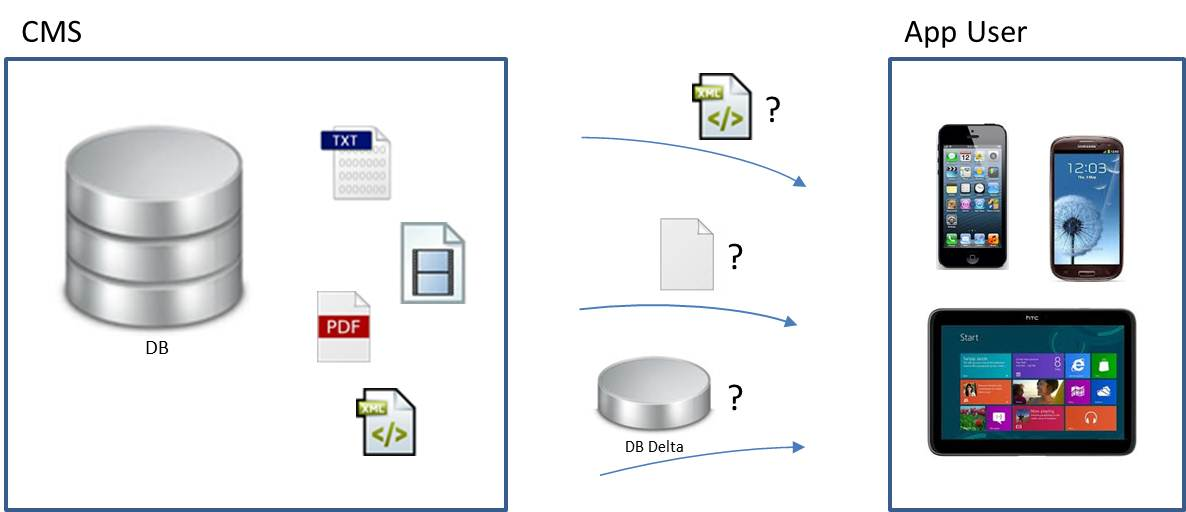
\includegraphics[width=0.70\textwidth]{graphics/titelbild.jpg}



\vspace{0.15\textheight}

Seminararbeit\\
ausgef�hrt an der\\ \vspace{0.3 cm}
Z�rcher Hochschule f�r Angewandte Wissenschaften (ZHAW)\\
Studiengang Informatik\\ \vspace{0.3 cm}
im Seminar "Handheld"\\ \vspace{0.3 cm}
unter der Leitung von\\
Christian Vils
\end{center}
\end{titlepage}

\cleardoublepage
\pagenumbering{roman}   % i, ii, iii, iv, ...
\setcounter{page}{1}
\cleardoublepage
\tableofcontents			%Inhaltsverzeichnis
\cleardoublepage
\cleardoublepage
\pagestyle{headings}
\pagenumbering{arabic}  % 1, 2, 3, 4, ...
\setcounter{page}{1}
\chapter{Projektinformationen}


\section{Ausgangslage}

F�r content-basierte Mobile Apps m�ssen immer wieder neue Inhalte publiziert werden. Dies soll jeweils vom Betreiber der App auf
einfache Art m�glich sein. Dies ist m�glich, wenn die Inhalte in einem CMS verwaltet werden. Die App soll automatisch aktuell gehalten
werden, ohne dass die ganze App aktualisiert werden muss, und auch ohne dass der Konsument aktiv wird. Wichtig ist zudem, dass die
Daten auch offline zur Verf�gung stehen und auch gr�ssere Datenmengen unproblematisch �bermittelt werden k�nnen. Trotzdem
muss aber ein Mechanismus gefunden werden, dass nur m�glichst kleine Datenmengen �bermittelt werden m�ssen um z.B. auf
geringe Bandbreite reagieren zu k�nnen, oder Roaming-Geb�hren klein zu halten. Zum Beispiel m�ssen Apps von Museen, Ausstellungen, Konzertbetreibern oder Zeitschriften diese Anforderungen erf�llen

\section{Aufgabenstellung / Abgrenzung}


\section{Ziele der Arbeit}

Das Ziel der Seminararbeit ist es aufzuzeigen, welche Systeme, Prozesse und Design-Patterns wichtig sind und in Frage kommen um den oben genannten Anforderungen gerecht zu werden. Insbesondere die Schwierigkeit, m�glichst effizient aktuelle Daten dem App-Benutzer zur Verf�gung zu stellen soll dabei beachtet werden.

Falls m�glich k�nnen bereits gewisse Teile praktisch umgesetzt werden: z.B. kann ein CMS bereitgestellt werden, �ber welches der Betreiber der App die Inhalte bereitstellen und zur Aktualisierung f�r die App freigeben kann. Weiter kann eine App entwickelt werden, welche ihre Inhalte �ber das CMS bezieht und die definier 

\section{Motivation}
W�re doch nur die Motivation da...
...
...


\section{Projektverlauf}

blablabla...
....
...


\begin{itemize}
\item Punkt1
\item ...

\end{itemize}


\section{Hilfsmittel}

Um m�glichst effizient programmieren zu k�nnen, haben wir als Entwicklungsumgebung Eclipse \cite{Eclipse} gew�hlt.
\newline
\\Um eine \emph{Versionskontrolle} zu haben, und damit wir beide gleichzeitig am Projekt arbeiten konnten, haben wir bei Github \cite{Github} ein Repository erstellt und s�mtliche f�r das Projekt n�tigen Dateien dort eingecheckt.
\newline
\\Die Dokumentation haben wir mit \LaTeX{} erstellt.

Pencil Project \cite{pencilProject}

\chapter{Strukturen}


\section{Typ Definitionen}
\subsection{menu}
...
...

\subsection{title}
...
...

\subsection{text}
...
...

\subsection{png}
...
...



\section{Views}
...
...

\subsection{txt}
...
...

\subsection{maps}
...
...


\section{Datenstruktur}
...
...


\section{Dokumentstruktur}


\clearpage{\pagestyle{empty}\cleardoublepage}
\bibliographystyle{alphadin} %oder plainnatDeutsch (alphadin geht nicht mit natbib)amsalpha
\bibliography{literatur}
%\clearpage{\pagestyle{empty}\cleardoublepage}
%\printindex										%fuer den Index
\end{document}

